% 2015陕西理 q20 图1：椭圆 x^2/12+y^2/3=1，圆 M:(x+2)^2+(y-1)^2=5/2，AB为圆M直径且A,B在椭圆上
\usetikzlibrary{arrows.meta}
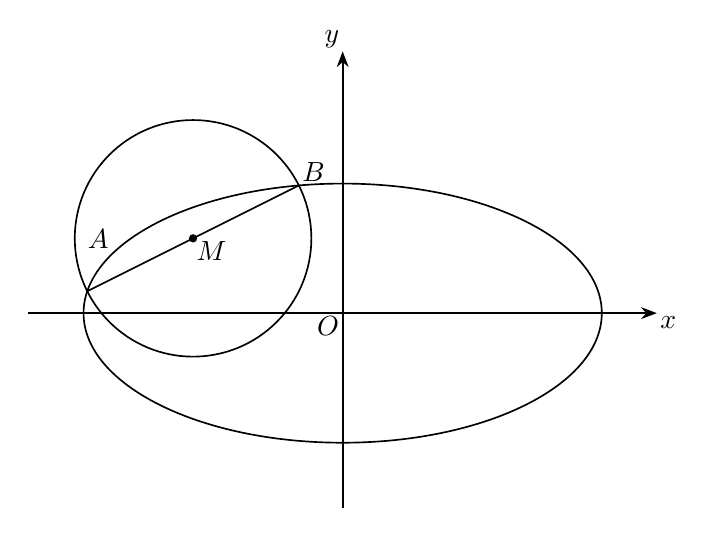
\begin{tikzpicture}[x=0.95cm,y=0.95cm,line width=.6pt,font=\normalsize,>=Stealth]
  \draw[->] (-4.2,0) -- (4.2,0) node[below right,inner sep=1pt] {$x$};
  \draw[->] (0,-2.6) -- (0,3.5) node[above left,inner sep=1pt] {$y$};
  \draw (0,0) ellipse [x radius=3.46410,y radius=1.73205];
  \draw (-2,1) circle [radius=1.58114];
  \draw (-3.41421,0.29289) -- (-0.58579,1.70711);
  \fill (-2,1) circle (1.5pt);
  \node[below left,inner sep=1pt] at (0,0) {$O$};
  \node[above,inner sep=1pt,xshift=4pt,yshift=14pt] at (-3.41421,0.29289) {$A$};
  \node[above right,inner sep=1pt] at (-0.58579,1.70711) {$B$};
  \node[below right,inner sep=1pt] at (-2,1) {$M$};
\end{tikzpicture}
